%!TEX program = xelatex
% Note: this template must be compiled with XeLaTeX rather than PDFLaTeX
% due to the custom fonts used. The line above should ensure this happens
% automatically, but if it doesn't, your LaTeX editor should have a simple toggle
% to switch to using XeLaTeX.

\documentclass[
  aspectratio=169, % Uncomment to use an aspect ratio of 16:9 (160 mm by 90 mm)
  %aspectratio=43, % Uncomment to use an aspect ratio of 4:3 (128mm by 96mm)
  t, % Top align all slide content by default
  onlytextwidth, % Typeset content in columns at text width
  10pt, % Default font size, use 10pt for the 16:9 aspect ratio and 8pt for the 4:3 aspect ratio
]{beamer}

\usepackage{../../ImperialTheme/beamer/beamerthemeImperial} % Use the Imperial theme

\def\imagefolder{../../ImperialTheme/beamer/Images}
\def\Rey{\text{Re}}
\title{Torus diagram + SPOD} % Presentation title to appear on the title slide and left footers

\subtitle{} % Presentation subtitle to appear on the title slide

\author{Víctor Ballester} % Author name(s) to appear on the title slide

\date{\today} % Presentation date to appear on the title slide and right footers

\begin{document}

\begingroup
\setbeamercolor{background canvas}{bg=ICLLightGrey} % Slide background color
\setbeamercolor{title page title}{fg=ICLBlue} % Title text color
\setbeamercolor{title page subtitle}{fg=ICLBlue} % Subtitle text color
\setbeamercolor{author}{fg=ICLBlue} % Author(s) text color
\setbeamercolor{date}{fg=ICLBlue} % Date text color
\setbeamertemplate{title page}[logo]{\imagefolder/ICL_Logo_Blue.pdf} % Imperial logo color, use 'ICL_Logo_White.pdf' for white and 'ICL_Logo_Blue.pdf' for blue
\frame[plain, s]{\titlepage} % Output the title page with no footer ('plain') and vertically distributed text ('s')
\endgroup

\begin{frame}
	\frametitle{Reminder}
	\centering

	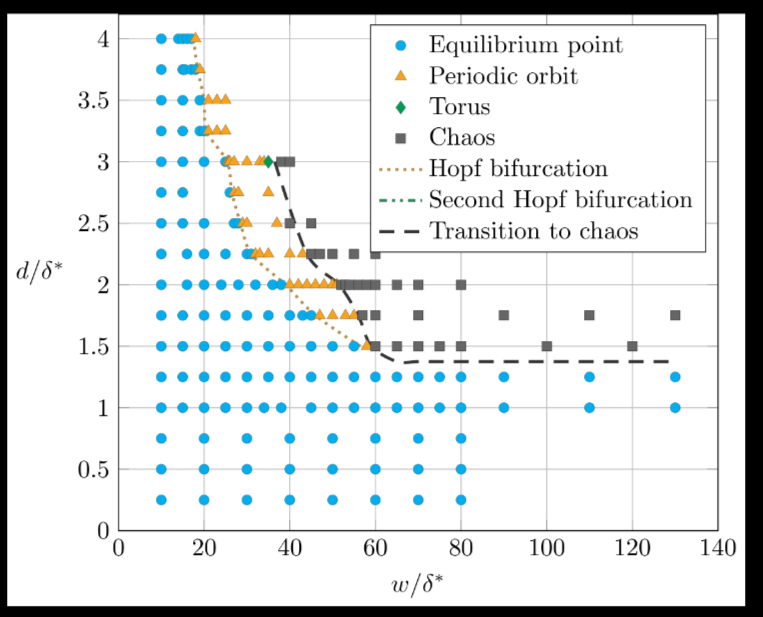
\includegraphics[width=0.5\linewidth]{Images/stabilitycurve.png}
\end{frame}
\begin{frame}
	\frametitle{Edge state analysis for $d=3$}
	\begin{itemize}
		\item As we approach the Hopf bifurcation at $w\sim 25.4$, the energy of this other periodic orbit increases, so I think those two states are unrelated.
		\item The L2 energy of the periodic orbit at $w=26$ is very low (of course, because it is only localized near the gap) around $0.47$.
		\item Also I think there are many more weird attractors wiothout a clear pattern than just the ones drawn in the previous diagram. because for some reason $w=16$ behaves differently than the other cases.
	\end{itemize}

\end{frame}
\begin{frame}
  \frametitle{Edge state energy}
	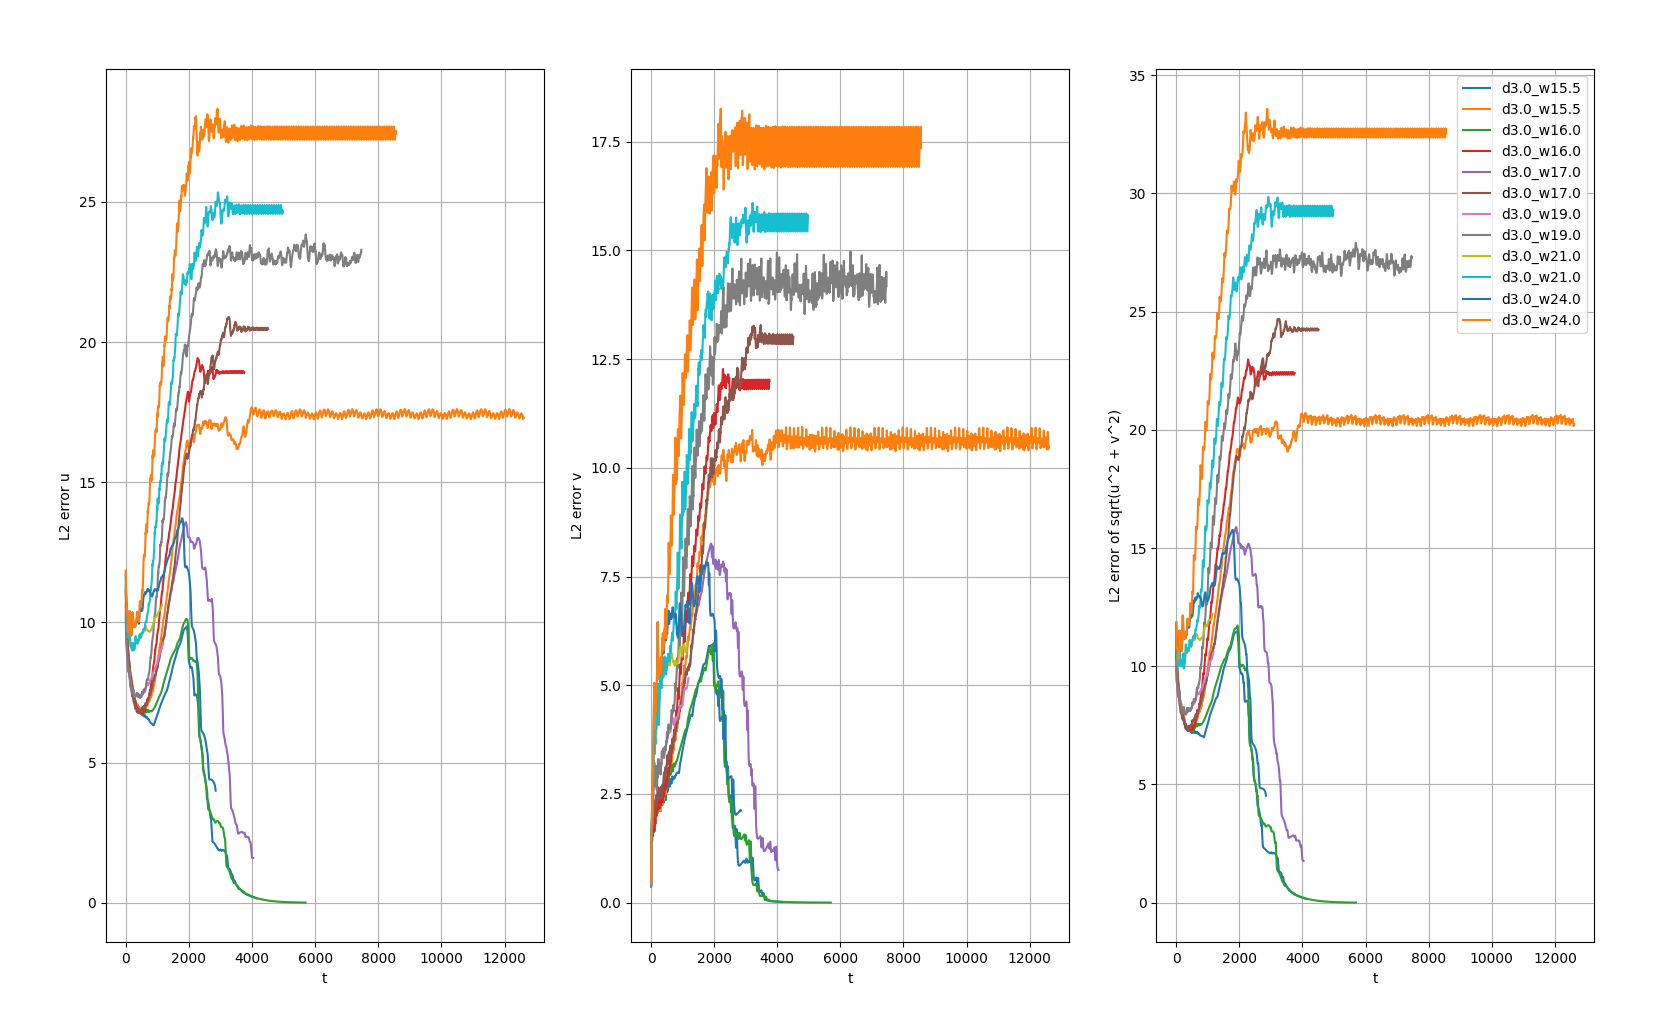
\includegraphics[width=0.8\linewidth]{Images/edgeStates.png}
  
\end{frame}
\begin{frame}
  \frametitle{P.O. full BL excited at $d=3$ and $w=21$}

	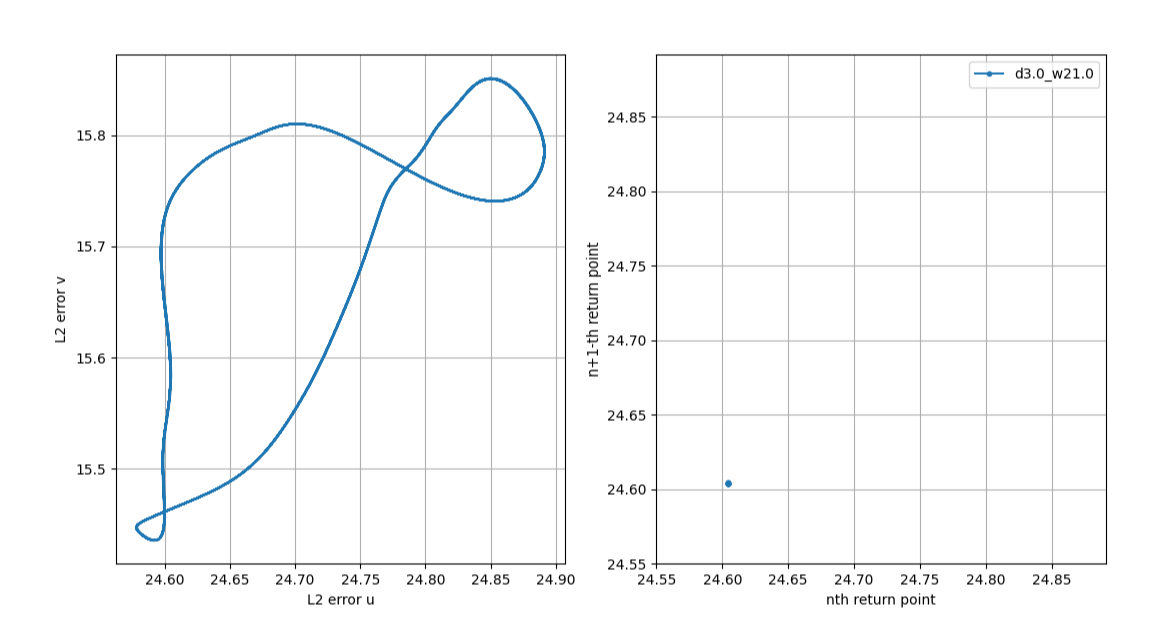
\includegraphics[width=0.8\linewidth]{Images/pod3_w21.png}
  
\end{frame}
\begin{frame}
  \frametitle{quasi-periodic? full BL excited at $d=3$ and $w=15.5$}

  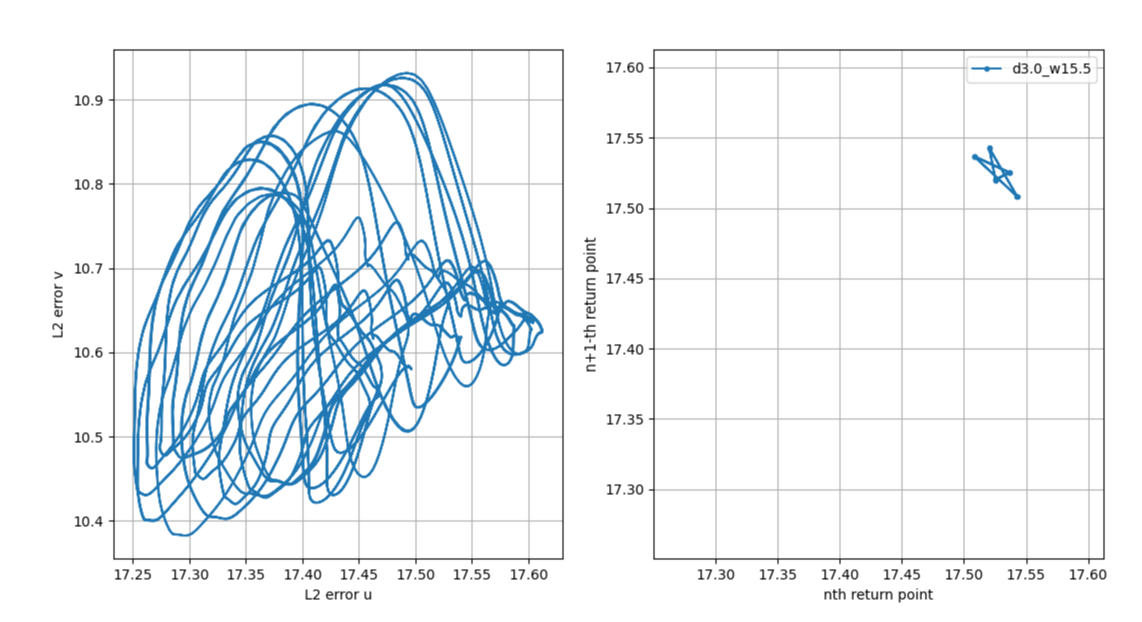
\includegraphics[width=0.8\linewidth]{Images/quasiPd3w15.5.png}
  
\end{frame}
\begin{frame}
  \frametitle{u fields}
	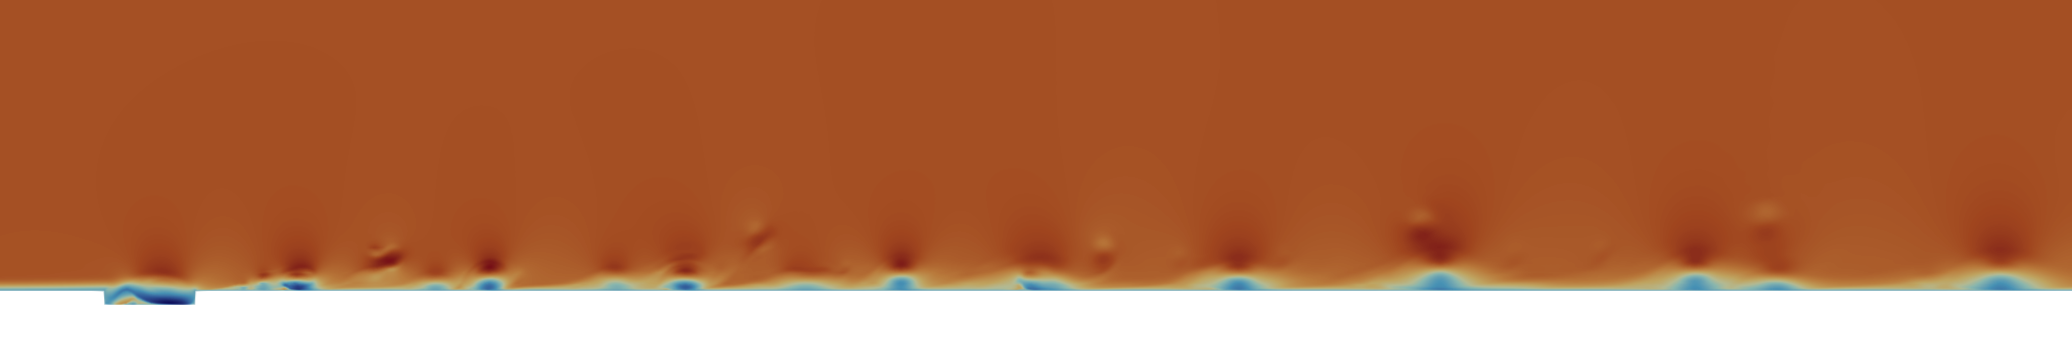
\includegraphics[width=\linewidth]{Images/field1.png}
	
\includegraphics[width=\linewidth]{Images/field2.png}
	
\includegraphics[width=\linewidth]{Images/field3.png}
  
\end{frame}
\begin{frame}
	\frametitle{SPOD analysis}
	
  	\begin{columns}[T] % [T] ensures correct vertical alignment
		\begin{column}{0.45\linewidth} % Left column
			\begin{itemize}
				\item Main mode: $A= 5170$, $\omega =0.107$.
				\item Second mode: $A = 620$, $ \omega = 0.055$.
			\end{itemize}
		\end{column}
		\begin{column}{0.54\linewidth} % Left column
			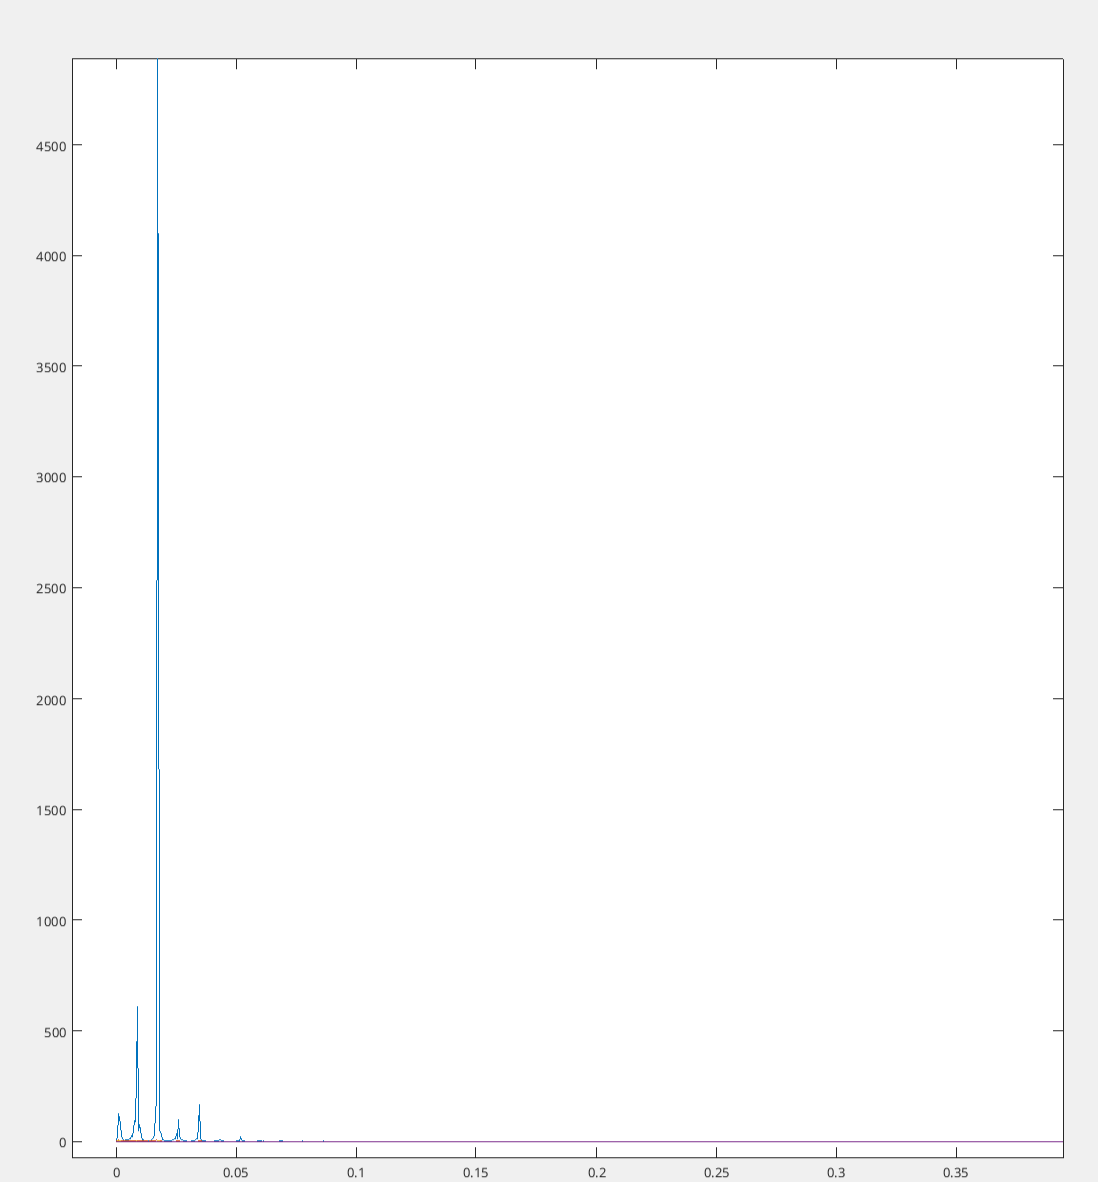
\includegraphics[width=0.8\linewidth]{Images/freqsSPOD.png}
		\end{column}
	\end{columns}
\end{frame}
\begin{frame}
  \frametitle{SPOD 1st mode u}
	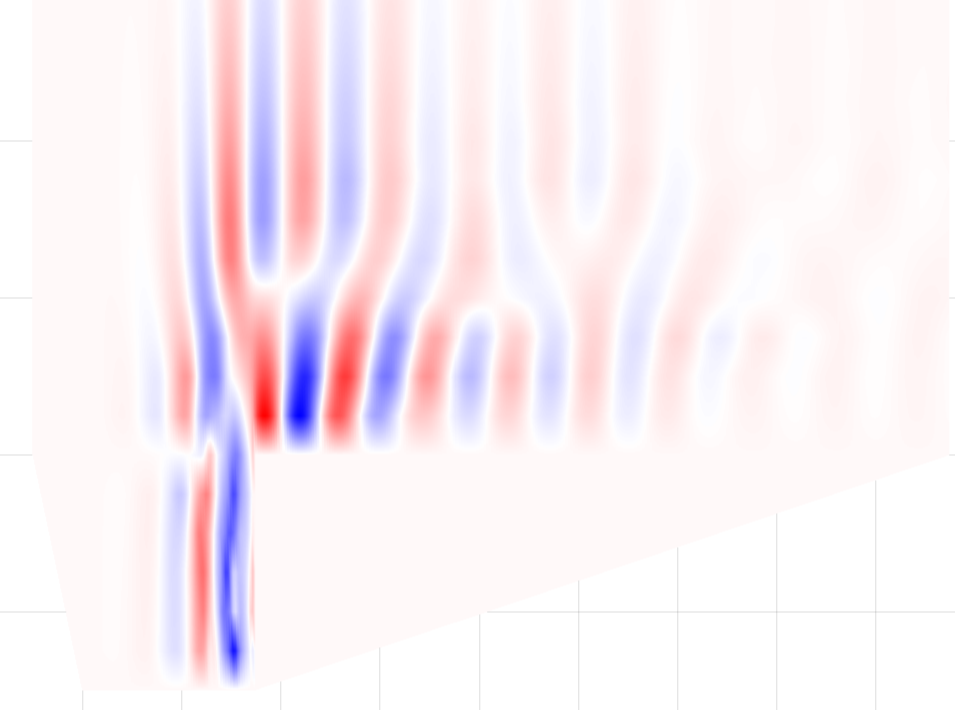
\includegraphics[width=0.6\linewidth]{Images/1stu.png}
  
\end{frame}
\begin{frame}
  \frametitle{SPOD 1st mode v}
	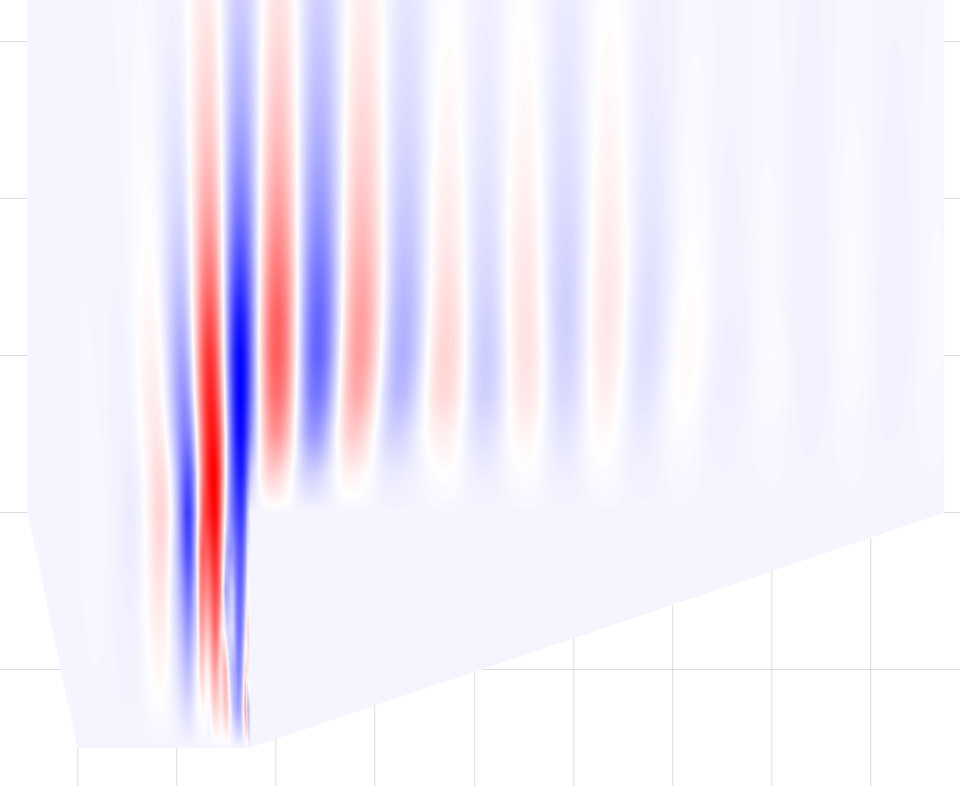
\includegraphics[width=0.6\linewidth]{Images/1stv.png}
  
\end{frame}
\begin{frame}
  \frametitle{SPOD 2nd mode u}
  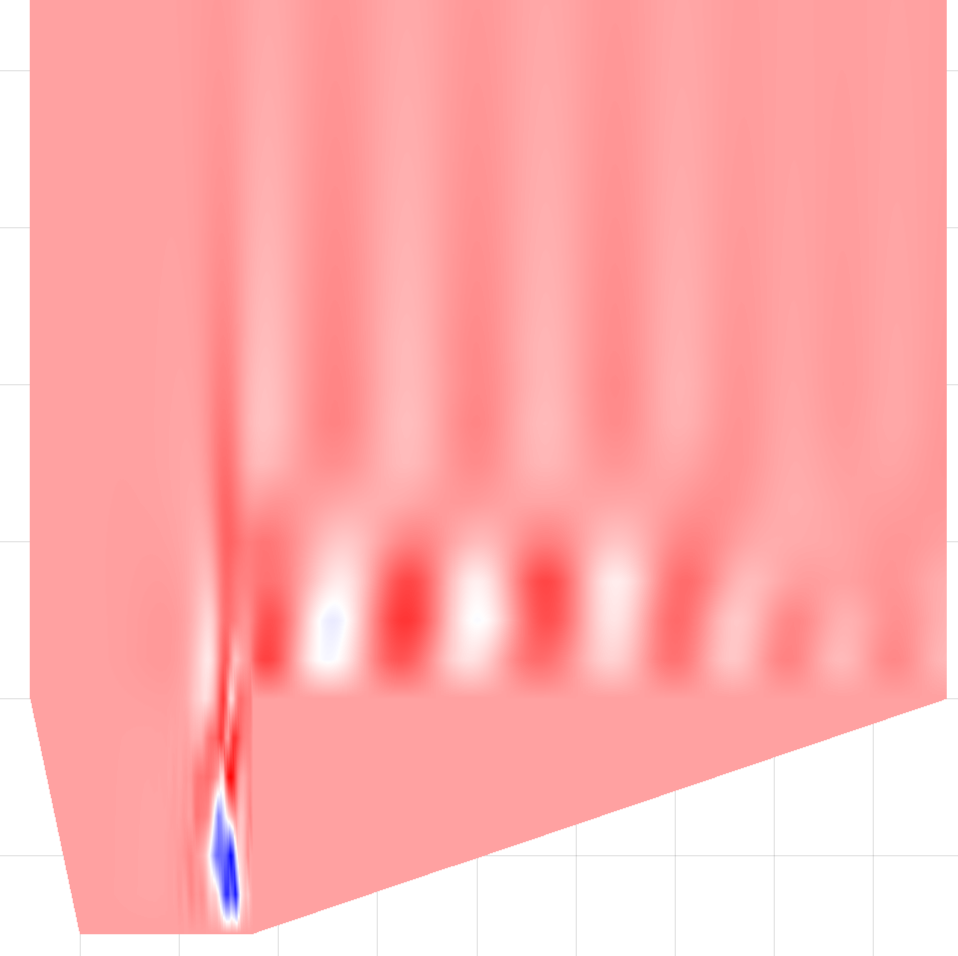
\includegraphics[width=0.5\linewidth]{Images/2ndu.png}
  
\end{frame}
\begin{frame}
  \frametitle{SPOD 2nd mode v}
  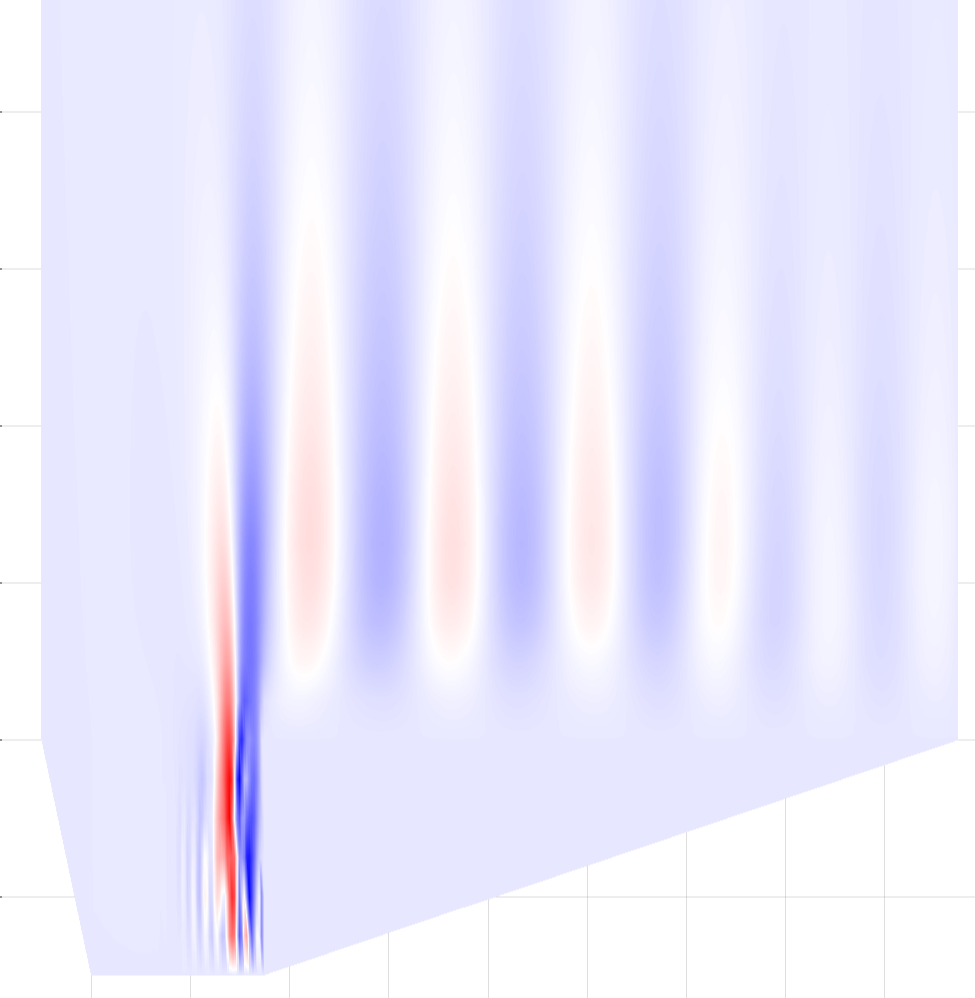
\includegraphics[width=0.5\linewidth]{Images/2ndv.png}
  
\end{frame}
\end{document}
